\documentclass{article}
\usepackage{tikz}
\usepackage{bm}
\usepackage{amsmath,amssymb}
\usetikzlibrary{positioning, arrows.meta, fit, shapes, decorations.pathreplacing}
\begin{document}
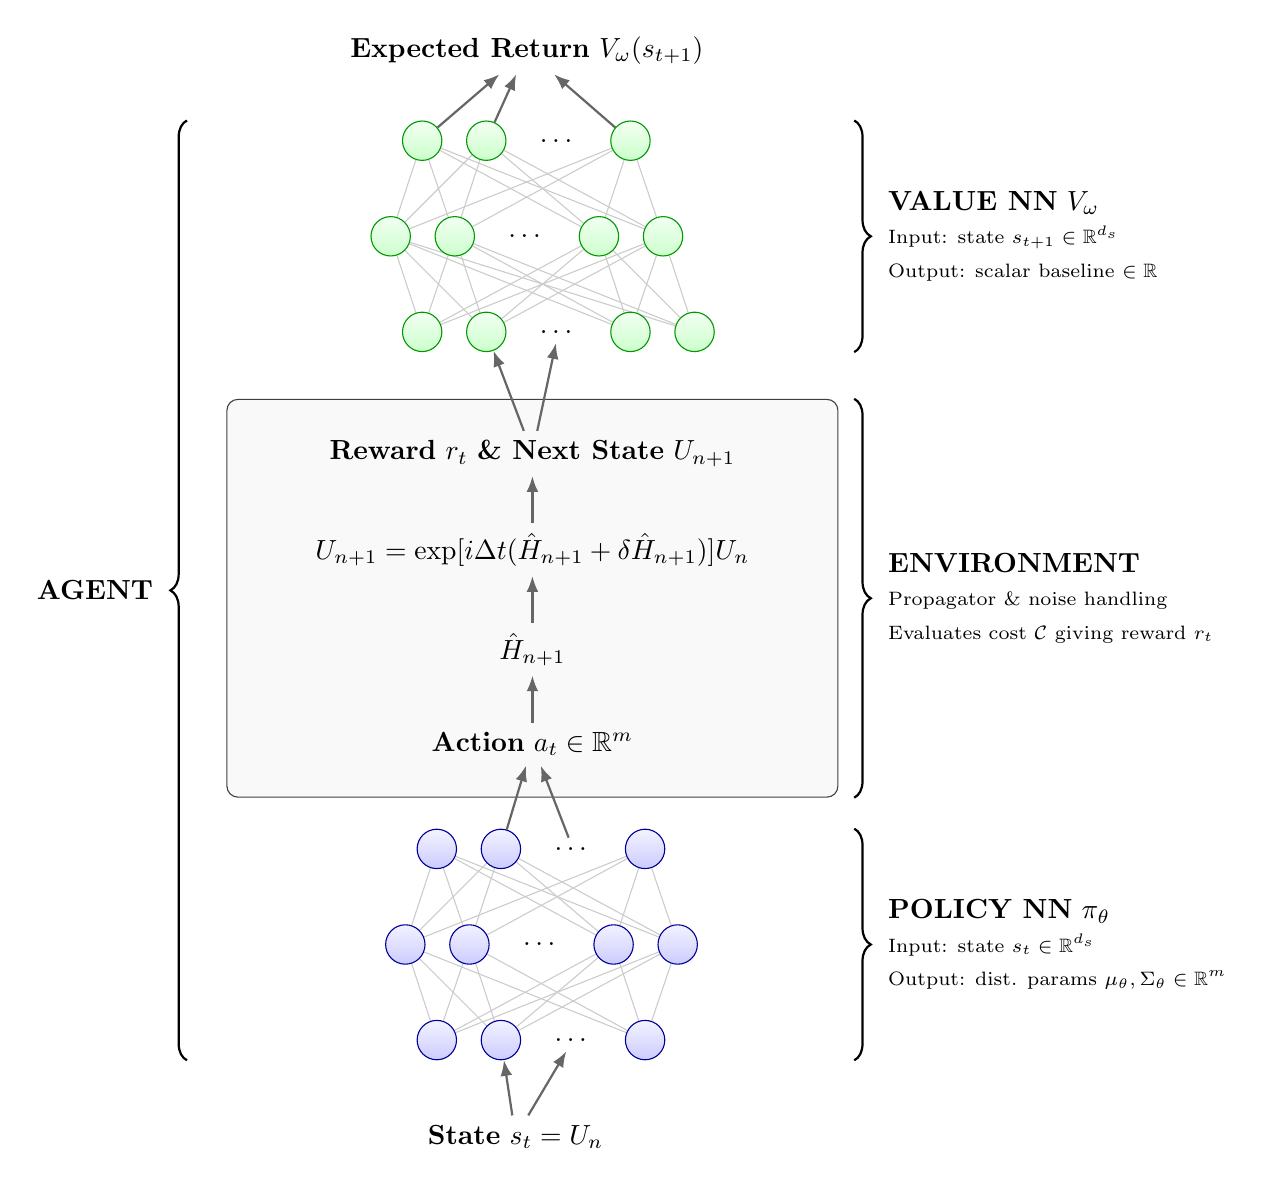
\begin{tikzpicture}[
    node distance=0.6cm and 0.6cm,
    bluenode/.style={circle, minimum size=0.5cm, inner sep=0pt, top color=blue!5, bottom color=blue!20, draw=blue!60!black},
    greennode/.style={circle, minimum size=0.5cm, inner sep=0pt, top color=green!5, bottom color=green!20, draw=green!60!black},
    envbox/.style={draw=gray!50!black, fill=gray!5, rounded corners, inner sep=10pt},
    arr/.style={-{Latex[length=2mm]}, thick, gray!80!black}
]

\pgfdeclarelayer{background}
\pgfsetlayers{background,main}

% Policy NN 
\node[align=center] (state) {\textbf{State} $s_t = U_n$};

\node[bluenode, above=0.7cm of state, xshift=-1cm] (p11) {};
\node[bluenode, right=0.3cm of p11] (p12) {};
\node[right=0.3cm of p12] (p1_dots) {$\dots$};
\node[bluenode, right=0.3cm of p1_dots] (p13) {};

\node[bluenode, above=0.7cm of p11, xshift=-0.4cm] (p21) {};
\node[bluenode, right=0.3cm of p21] (p22) {};
\node[right=0.3cm of p22] (p2_dots) {$\dots$};
\node[bluenode, right=0.3cm of p2_dots] (p23) {};
\node[bluenode, right=0.3cm of p23] (p24) {};

\node[bluenode, above=0.7cm of p21, xshift=0.4cm] (p31) {};
\node[bluenode, right=0.3cm of p31] (p32) {};
\node[right=0.3cm of p32] (p3_dots) {$\dots$};
\node[bluenode, right=0.3cm of p3_dots] (p33) {};

% Connections for Policy NN
\begin{pgfonlayer}{background}
\foreach \i in {1,2,3}
    \foreach \j in {1,2,3,4} {
        \draw[gray!40, thin] (p1\i) -- (p2\j);
    }
\foreach \i in {1,2,3,4}
    \foreach \j in {1,2,3} {
        \draw[gray!40, thin] (p2\i) -- (p3\j);
    }
\end{pgfonlayer}

\draw[arr] (state) -- (p12);
\draw[arr] (state) -- (p1_dots);

% Action
\node[above=0.8cm of p32, xshift=0.4cm, align=center] (action) {\textbf{Action} $a_t \in \mathbb{R}^m$};
\draw[arr] (p32) -- (action);
\draw[arr] (p3_dots) -- (action);

% Environment
\node[above=0.6cm of action, align=center] (H) {$\hat{H}_{n+1}$};
\node[above=0.6cm of H, align=center] (U) {$U_{n+1} = \exp[i\Delta t(\hat{H}_{n+1} + \delta\hat{H}_{n+1})]U_n$};
\node[above=0.6cm of U, align=center] (cost) {\textbf{Reward} $r_t$ \textbf{\& Next State} $U_{n+1}$};

\draw[arr] (action) -- (H);
\draw[arr] (H) -- (U);
\draw[arr] (U) -- (cost);

\begin{pgfonlayer}{background}
\node[envbox, fit=(action) (H) (cost) (U), inner xsep=1.0cm, inner ysep=0.4cm] (env) {};
\end{pgfonlayer}

% Value NN
\node[greennode, above=1.0cm of cost, xshift=-1.4cm] (v11) {};
\node[greennode, right=0.3cm of v11] (v12) {};
\node[right=0.3cm of v12] (v1_dots) {$\dots$};
\node[greennode, right=0.3cm of v1_dots] (v13) {};
\node[greennode, right=0.3cm of v13] (v14) {};

\node[greennode, above=0.7cm of v11, xshift=-0.4cm] (v21) {};
\node[greennode, right=0.3cm of v21] (v22) {};
\node[right=0.3cm of v22] (v2_dots) {$\dots$};
\node[greennode, right=0.3cm of v2_dots] (v23) {};
\node[greennode, right=0.3cm of v23] (v24) {};

\node[greennode, above=0.7cm of v21, xshift=0.4cm] (v31) {};
\node[greennode, right=0.3cm of v31] (v32) {};
\node[right=0.3cm of v32] (v3_dots) {$\dots$};
\node[greennode, right=0.3cm of v3_dots] (v33) {};

% Connections for Value NN
\begin{pgfonlayer}{background}
\foreach \i in {1,2,3,4}
    \foreach \j in {1,2,3,4} {
        \draw[gray!40, thin] (v1\i) -- (v2\j);
    }
\foreach \i in {1,2,3,4}
    \foreach \j in {1,2,3} {
        \draw[gray!40, thin] (v2\i) -- (v3\j);
    }
\end{pgfonlayer}

\draw[arr] (cost) -- (v12);
\draw[arr] (cost) -- (v1_dots);

\node[above=0.7cm of v3_dots, xshift=-0.4cm, align=center] (reward) {\textbf{Expected Return} $V_\omega(s_{t+1})$};
\draw[arr] (v31) -- (reward);
\draw[arr] (v32) -- (reward);
\draw[arr] (v33) -- (reward);

% Annotative Braces
\coordinate (agent_brace_bottom) at (env.south west |- p11.south);
\coordinate (agent_brace_top)    at (env.north west |- v33.north);
\draw[decorate, decoration={brace, amplitude=6pt}, thick] 
    ([xshift=-0.5cm]agent_brace_bottom) -- ([xshift=-0.5cm]agent_brace_top) 
    node[midway, left=0.3cm] {\textbf{AGENT}};

\coordinate (p_brace_bottom) at (env.south east |- p11.south);
\coordinate (p_brace_top)    at (env.north east |- p33.north);
\draw[decorate, decoration={brace, amplitude=6pt}, thick] 
    ([xshift=0.2cm]p_brace_top) -- ([xshift=0.2cm]p_brace_bottom) 
    node[midway, right=0.3cm, align=left] {
        \textbf{POLICY NN} $\pi_\theta$\\
        \textnormal{\scriptsize Input: state $s_t \in \mathbb{R}^{d_s}$}\\
        \textnormal{\scriptsize Output: dist. params $\mu_\theta, \Sigma_\theta \in \mathbb{R}^m$}
    };

\coordinate (v_brace_bottom) at (env.south east |- v11.south);
\coordinate (v_brace_top)    at (env.north east |- v33.north);
\draw[decorate, decoration={brace, amplitude=6pt}, thick] 
    ([xshift=0.2cm]v_brace_top) -- ([xshift=0.2cm]v_brace_bottom) 
    node[midway, right=0.3cm, align=left] {
        \textbf{VALUE NN} $V_\omega$\\
        \textnormal{\scriptsize Input: state $s_{t+1} \in \mathbb{R}^{d_s}$}\\
        \textnormal{\scriptsize Output: scalar baseline $\in \mathbb{R}$}
    };

\draw[decorate, decoration={brace, amplitude=6pt}, thick] 
    ([xshift=0.2cm]env.north east) -- ([xshift=0.2cm]env.south east) 
    node[midway, right=0.3cm, align=left] {
        \textbf{ENVIRONMENT}\\
        \textnormal{\scriptsize Propagator \& noise handling}\\
        \textnormal{\scriptsize Evaluates cost $\mathcal{C}$ giving reward $r_t$}
    };

\end{tikzpicture}
\end{document}